\iffalse
\def\mytitle{MATRICES USING PYTHON(CONIC)}
\def\myauthor{R.Radhika}
\def\contact{r170234@rguktrkv.ac.in}
\def\mymodule{Future Wireless Communication (FWC)}
\documentclass[10pt, a4paper]{article}
\usepackage[a4paper,outer=1.5cm,inner=1.5cm,top=1.75cm,bottom=1.5cm]{geometry}
\twocolumn
\usepackage{graphicx}
\graphicspath{{./images/}}
\usepackage[colorlinks,linkcolor={black},citecolor={blue!80!black},urlcolor={blue!80!black}]{hyperref}
\usepackage[parfill]{parskip}
\usepackage{lmodern}
\usepackage{tikz}
	\usepackage{physics}
%\documentclass[tikz, border=2mm]{standalone}
%\usepackage{karnaugh-map}
%\documentclass{article}
\usepackage{tabularx}
%\usepackage{circuitikz}
\usepackage{enumitem}
\usetikzlibrary{calc}
\usepackage{amsmath}
\usepackage{amssymb}
\renewcommand*\familydefault{\sfdefault}
\usepackage{watermark}
\usepackage{lipsum}
\usepackage{xcolor}
\usepackage{listings}
\usepackage{float}
\usepackage{titlesec}
\providecommand{\mtx}[1]{\mathbf{#1}}
\titlespacing{\subsection}{1pt}{\parskip}{3pt}
\titlespacing{\subsubsection}{0pt}{\parskip}{-\parskip}
\titlespacing{\paragraph}{0pt}{\parskip}{\parskip}
\newcommand{\figuremacro}[5]{
    \begin{figure}[#1]
        \centering
        \includegraphics[width=#5\columnwidth]{#2}
        \caption[#3]{\textbf{#3}#4}
        \label{fig:#2}
    \end{figure}
}

\newcommand{\myvec}[1]{\ensuremath{\begin{pmatrix}#1\end{pmatrix}}}
\let\vec\mathbf
\lstset{
frame=single, 
breaklines=true,
columns=fullflexible
}

\title{\mytitle}
\author{\myauthor\hspace{1em}\\\contact\\FWC22066\hspace{6.5em}IITH\hspace{0.5em}\mymodule\hspace{6em}Assignment}
\begin{document}
	\maketitle
	\tableofcontents
   \section{Problem}
   \fi
Find   the area bounded by the curve $y=x|x|, x$-axis and the ordinates $x$=-1 and $x$=1.
\\
\solution 
	\begin{figure}[!h]
		\centering
 \includegraphics[width=\columnwidth]{chapters/12/8/3/17/figs/conicfig.pdf}
		\caption{}
		\label{fig:12/8/3/17}
  	\end{figure}
   \iffalse
[Hint: y=$x^2$ if $x>0$  and y=$-x^2$ if $x<0$]
   					
\section{Construction}
  \includegraphics[scale=0.47]{conicfig.pdf}
  	\begin{center}
  Figure of construction
  	\end{center}
  \section{Solution}
  
\raggedright\large{ Draw the ordinates by using $x$=1 and $x$=-1. Then we need to draw  two parabolas using  given hint [Hint: y=$x^2$ if $x>0$  and y=$-x^2$ if $x<0$]for that we need to find out the area bounded by the curve  y=$x|x|$  .}
\vspace{2mm}\\
\raggedright\large{Then the limits from -1 to 1  and the points(-1,-1),(1,1)}\vspace{2mm}\\
The standard conic equation\\
\begin{align}
\vec{x}^{\top}\vec{V}\vec{x}+2\vec{u}^{\top}\vec{x}+f=0
\end{align}
\begin{align}
\vec{x}^{\top}\vec{V}\vec{x}+2\vec{u_1}^{\top}\vec{x}+f_1=0
\end{align}
\fi
The parameters of the given conics are
\begin{align}
	\vec{V}_1&=\myvec{1&0\\0&0} ,\vec{u_1}=\myvec{0\\-\frac{1}{2}},  f_1=0
	\\
	\vec{V}_2&=\myvec{-1&0\\0&0} ,\vec{u_2}=\myvec{0\\-\frac{1}{2}},  f_2=0
\end{align}
The determinant equation for the intersection of two conics is 
\iffalse
\begin{align}
|\myvec{\vec{V_1}+\mu{\vec{V_2}}&\vec{u_1}+\mu{\vec{u_2}}\\\vec{u_1}+\mu{\vec{u_2}}&0}|
\end{align}
substitute eq 3 and 4 in eq 6\\
\fi
\begin{align}
\mydet{1-\mu&0&0\\0&0&-\frac{1}{2}-\frac{\mu}{2}\\0&-\frac{1}{2}-\frac{\mu}{2}&0} = 0
\end{align}
yielding,
\begin{align}
	\mu^3+\mu^2-\mu-1&=0
	\\
	\implies
	\mu&=-1, 1, 1
\end{align}
\iffalse
\begin{align}
|\vec{V_1}+\mu\vec{V_2}|<0
\end{align}
substitute $\vec{V_1}$ and $\vec{V_2}$ in eq-9\\
we get 0\\
\begin{align}
\vec{x}=\vec{q}+\mu{\vec{m}}
\end{align}
\begin{align}
q=\vec{V^{-1}}(k\vec{n}-\vec{u})
\end{align}
\begin{align}
k=\pm\sqrt{\frac{\norm{\vec{u_2}}^2\vec{V}-f}{\vec{n}^{\top}\vec{V^{-1}}\vec{n}}}
\end{align}
$\vec{n}=\myvec{1\\-1}$\\
$\vec{m}=\myvec{1\\1}$\\

by solving eq 10 and 11 we get\\
\begin{align}
\vec{q}=\myvec{0\\0}
\end{align}


 Given equation :  y=$x|x|$\\

We know that \\
\begin{equation}
   |x| =
    \begin{cases}
      x, & {x\geq0}\\
      -x & {x<0}\\
    \end{cases}       
\end{equation}

	Therefore,
\begin{equation}
   y=x|x| =
    \begin{cases}
      xx, & {x\geq0}\\
      x(-x) & {x<0}\\
    \end{cases}       
\end{equation}
\begin{equation}
   y =
    \begin{cases}
      x^2, & {x\geq0}\\
      -x^2 & {x<0}\\
    \end{cases}       
\end{equation}
Area Required=Area ABO+Area DCO\\
\textbf{Area of DCO}

Area  : \[ \int_{-1}^{1} y \,dx \]

Here, y=$x|x|$

Therefore Area DCO: \[ \int_{-1}^{0} -x^2 \,dx \]

 yielding ,\\
 
   -1/3 \\
 
 $|(-1/3)|$=1/3\\
 
 Area of DCO= 1/3

\textbf{Area  of ABO}: \[ \int_{0}^{1} x^2 \,dx \]

    yielding 1/3\\
   
     
     Area of ABO= 1/3
     

\textbf{Required Area=ABO+DCO}:
  1/3+1/3=2/3
Below python code realizes the above construction 

\begin{table}[h!]
    \begin{tabular}{|c|}
    \hline
         https://github.com/Radhikarkv/fwcproject.git\\
	\hline
    \end{tabular}
\end{table}
\end{document}
\fi
